\documentclass[conference]{IEEEtran}

\usepackage{cite}
\usepackage{amsmath,amssymb,amsfonts}
\usepackage{algorithm}
\usepackage{algpseudocode}
\usepackage{graphicx}
\usepackage{textcomp}

\begin{document}

\title{Implementación y Análisis Experimental del Algoritmo de Gale--Shapley}

\author{
\IEEEauthorblockN{Juan Pablo González-Mendoza}
\IEEEauthorblockA{
Departamento de Robótica y Mecatrónica\\
Centro de Investigación en Computación, IPN\\
Ciudad de México, México\\
jgonzaleza26@cic.mx}
}

\maketitle

\begin{abstract}
En este trabajo se presenta la implementación y análisis experimental del algoritmo de emparejamiento estable de Gale--Shapley. Se desarrolla un generador de instancias sintéticas para evaluar el comportamiento del algoritmo bajo diferentes tamaños de entrada y modos de propuesta. Asimismo, se comparan implementaciones en Python y C++ con el objetivo de validar empíricamente la complejidad teórica $O(n^2)$ y analizar el impacto del lenguaje en el rendimiento computacional.
\end{abstract}\vspace{0.5cm}

\begin{IEEEkeywords}
Emparejamiento estable, Gale--Shapley, complejidad computacional, análisis experimental, C++, Python.
\end{IEEEkeywords}

\section{Introducción}

El problema del emparejamiento estable, formulado por Gale y Shapley, consiste en encontrar una asignación entre dos conjuntos de igual tamaño tal que no exista un par que prefiera mutuamente emparejarse entre sí antes que con sus parejas actuales. Este problema posee aplicaciones en asignación de plazas médicas, sistemas de admisión y plataformas digitales de recomendación.\\

\noindent El objetivo de este trabajo es implementar el algoritmo clásico de Gale--Shapley, generar instancias controladas y analizar empíricamente su desempeño en Python y C++.

\section{Metodología}

\begin{figure}[h]
    \centering
    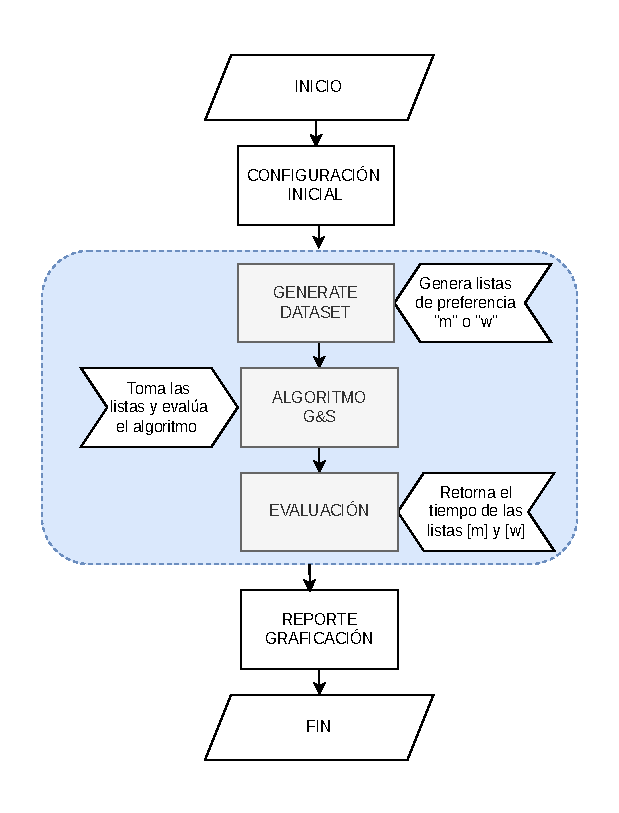
\includegraphics[width=0.4\textwidth]{Diagrams/D2.pdf}
    \caption{Diseño de implemenación del algoritmo Gale and Shappley}
    \label{fig:D2}
    \ref{fig:D2}
\end{figure}

\subsection{Generación de Instancias}

\noindent Para garantizar reproducibilidad, se desarrolló un generador de instancias que produce perfiles de preferencias aleatorias. El usuario digíta \textit{"m"} para referirse a preferencia a los hombres y \textit{"w"} a las mujeres. El orden de preferencia se escoge aleatoriamente como se mencionó antes.

\begin{algorithm}
\caption{Generación de Instancias de Emparejamiento}
\begin{algorithmic}[1]
\Procedure{GenerateDataset}{$n, mode, s$}
    \State Inicializar generador aleatorio $s$
    \State Definir conjuntos $H=\{H_0,\dots,H_{n-1}\}$ y $W=\{W_0,\dots,W_{n-1}\}$
    \State Crear lista $\mathcal{L}$ con $n$ y $mode$
    \If{$mode = \texttt{"m"}$}
        \ForAll{$h \in H$}
            \State Generar permutación aleatoria de $W$
        \EndFor
        \ForAll{$w \in W$}
            \State Generar permutación aleatoria de $H$
        \EndFor
    \Else
        \ForAll{$w \in W$}
            \State Generar permutación aleatoria de $H$
        \EndFor
        \ForAll{$h \in H$}
            \State Generar permutación aleatoria de $W$
        \EndFor
    \EndIf
    \State Serializar y guardar en archivo .txt
\EndProcedure
\end{algorithmic}
\end{algorithm}
\vspace{0.5cm}

Ejemplo de salida:\\

\begin{verbatim}
3
m
H0  M2  M0  M1
H1  M0  M2  M1
H2  M1  M0  M2
M0  H1  H0  H2
M1  H0  H2  H1
M2  H2  H1  H0
\end{verbatim}

\noindent En es

\subsection{Algoritmo de Gale--Shapley}

\begin{algorithm}
\caption{Algoritmo Gale--Shapley}
\begin{algorithmic}[1]
\Procedure{GaleShapley}{$n, Pref_P, Rank_R$}
    \State Inicializar arreglos de emparejamiento
    \State Conjunto $F$ de proponentes libres
    \While{$F \neq \emptyset$}
        \State Seleccionar $p \in F$
        \State $r \gets$ siguiente preferencia de $p$
        \If{$r$ está libre}
            \State Emparejar $p$ con $r$
        \Else
            \State Comparar rangos y actualizar emparejamiento si es necesario
        \EndIf
    \EndWhile
    \State Retornar emparejamiento
\EndProcedure
\end{algorithmic}
\end{algorithm}

\begin{table}[H]
\centering
\caption{Ejecución del Algoritmo}
\begin{tabular}{|c|l|l|}
\hline
\textbf{Ronda} & \textbf{Propuesta} & \textbf{Resultado} \\
\hline
1 & H0 $\to$ M2 & M2 libre $\Rightarrow$ acepta. (H0,M2) \\
2 & H1 $\to$ M0 & M0 libre $\Rightarrow$ acepta. (H1,M0) \\
3 & H2 $\to$ M1 & M1 libre $\Rightarrow$ acepta. (H2,M1) \\
\hline
\multicolumn{3}{|c|}{\textbf{Resultado final: (H0,M2) (H1,M0) (H2,M1)}} \\
\hline
\end{tabular}
\end{table}

\section{Resultados Experimentales}

Se realizaron pruebas para diferentes valores de $n$ en ambos lenguajes. Las gráficas generadas muestran crecimiento cuadrático del tiempo de ejecución, confirmando la complejidad teórica.

\begin{figure}[ht]
\centering
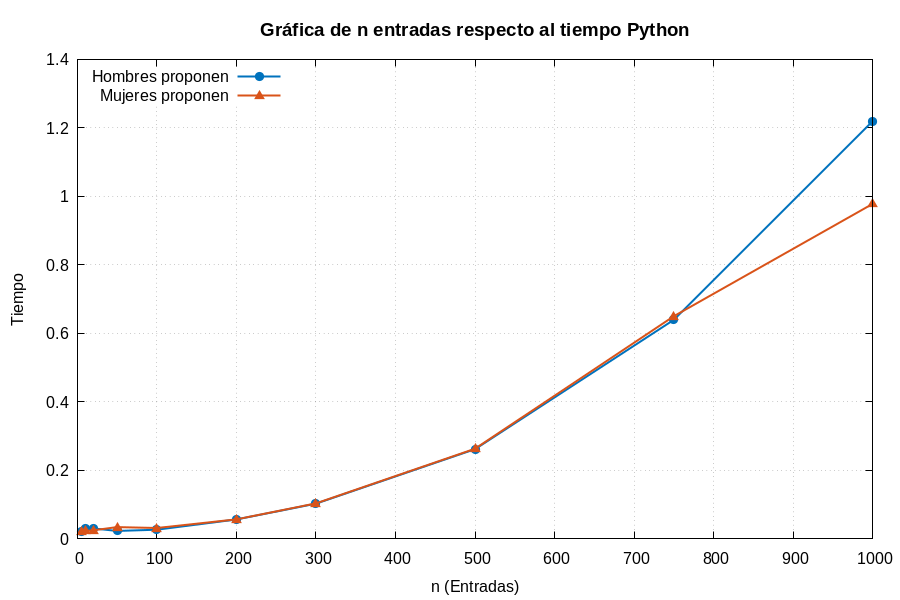
\includegraphics[width=0.45\textwidth]{Diagrams/graph_Python.png}
\caption{Tiempo de ejecución en Python}
\end{figure}

\begin{table}[!t]
\centering
\caption{Benchmark algoritmo Gale-Shapley - Python\\
\small Repeticiones: 3 \quad }
\label{tab:benchmark-gale-shapley}
\begin{tabular}{|r|c|c|}
\hline
$n$ & H-proponen (s) & M-proponen (s) \\
\hline
5    & 0.023699 & 0.032120 \\
10   & 0.024672 & 0.020448 \\
20   & 0.031284 & 0.024579 \\
50   & 0.024796 & 0.030515 \\
100  & 0.031187 & 0.036778 \\
200  & 0.059790 & 0.054848 \\
300  & 0.103847 & 0.113359 \\
500  & 0.272918 & 0.281324 \\
750  & 0.587009 & 0.563379 \\
1000 & 1.047477 & 1.048449 \\
\hline
\end{tabular}
\end{table}


\begin{figure}[ht]
\centering
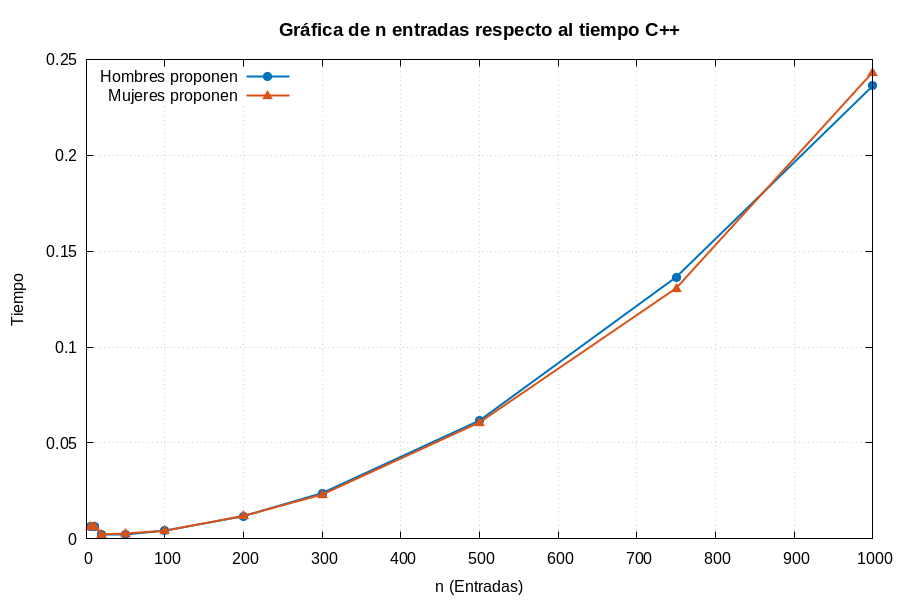
\includegraphics[width=0.45\textwidth]{Diagrams/graph_C++.png}
\caption{Tiempo de ejecución en C++}
\end{figure}


\begin{table}[!t]
\centering
\caption{Benchmark algoritmo Gale-Shapley - C++\\
\small Repeticiones: 3 \quad }
\label{tab:benchmark-gale-shapley-cpp}
\begin{tabular}{|r|c|c|}
\hline
$n$ & H-proponen (s) & M-proponen (s) \\
\hline
5    & 0.002449 & 0.002837 \\
10   & 0.004161 & 0.002323 \\
20   & 0.004438 & 0.003813 \\
50   & 0.003754 & 0.003109 \\
100  & 0.007666 & 0.003685 \\
200  & 0.013377 & 0.011594 \\
300  & 0.026677 & 0.029002 \\
500  & 0.070004 & 0.065064 \\
750  & 0.148317 & 0.150865 \\
1000 & 0.259636 & 0.263006 \\
\hline
\end{tabular}
\end{table}

Los resultados muestran que C++ presenta una mejora significativa en tiempos de ejecución respecto a Python, especialmente para valores grandes de $n$.


\begin{table}[!t]
\centering
\caption{Tiempos de ejecución por tarea -- Gale--Shapley Python\\
\small $n = 500$, modo: H-proponen}
\label{tab:tiempos-tareas}
\begin{tabular}{|l|c|c|}
\hline
Tarea & Tiempo (s) & (\%) \\
\hline
Lectura stdin         & 0.001823 & 0.6 \\
Init estructuras      & 0.000412 & 0.1 \\
Lectura preferencias  & 0.089341 & 31.2 \\
Conversión nombres→ID & 0.124876 & 43.6 \\
Gale--Shapley         & 0.065209 & 22.8 \\
Salida                & 0.004812 & 1.7 \\
\hline
\textbf{TOTAL} & \textbf{0.286473} & \textbf{100.0} \\
\hline
\end{tabular}
\end{table}


\section{Análisis de Complejidad}
El algoritmo garantiza terminación debido a que cada proponente avanza estrictamente en su lista de preferencias. En el peor caso, cada uno realiza $n$ propuestas, resultando en una complejidad $O(n^2)$.

Asimismo, el emparejamiento obtenido es estable y óptimo para el grupo proponente.



\section{Conclusiones}

Este reporte presentó la implementación y comparación del algoritmo de emparejamiento estable en dos lenguajes de programación, evaluando su rendimiento mediante diversas entradas y etapas de procesamiento. El objetivo fue determinar la conveniencia del uso de cada lenguaje según el contexto de la aplicación, concluyendo que la elección depende de los requisitos de eficiencia; específicamente, para tareas que demandan procesamiento rápido de información, \texttt{C++} ofrece ventajas significativas en tiempo de ejecución. Aunque la implementación en \texttt{Python} resultó más sencilla, \texttt{C++} proporcionó un control más preciso sobre la gestión de memoria y la sintaxis, a pesar de los desafíos de configuración encontrados en la plataforma \texttt{COACH}. El desarrollo de este trabajo permitió validar la complejidad teórica mediante pruebas empíricas, reforzando la importancia de las estructuras de datos y el manejo adecuado de librerías para la medición de tiempos y generación de archivos de análisis.
\end{document}